%!TEX root = umthsmpl.tex
\chapter{A model of location privacy and utility}
\label{ch1}

Many current models of location privacy primarily model threats from location based services, and propose defenses based on differential privacy strategies~\cite{andres2013geo,ho2011differential}.
However, the strategies studied in these works involve a service provider obfuscating databases of location logs, which requires the user to trust the service; this is not applicable from the point of a user who does not trust the service. 
In this chapter, I plan to generalize an existing method of quantifying location privacy~\cite{shokri2011quantifying}, and extend it to allow for threats from non-LBS usage. In my preliminary work, I present a novel framework to identify a user from both location profiling (LP) and trajectory linking (TL).
%I look at potential vectors for attacking location privacy, and argue for an economic model of privacy. I also
I propose to investigate game theoretic~\cite{freudiger2009non} and information theoretic models~\cite{sankar2013utility} to capture the varying worth of location privacy depending on the user and location. I will also evaluate the accuracy of the LP/TL framework and these models using a synthetic dataset created from a field survey. I will seek additional datasets as well.

\section{Preliminary work: Framework for location profiling and trajectory linking}
% I employ a utility model to quantify location privacy. 
I summarize the different adversaries and types of threats against location privacy. Next, I develop a general model of location profiling and trajectory linking that can be used in various ways by these attackers. Finally, I evaluate some simple location profiling and trajectory linking algorithms.
%Next, I formalize the framework behind several of these problems. I then discuss several possible scenarios and how they fit in this framework. Finally, I evaluate the risk-privacy balance with respect to a mobility dataset.

\paragraph*{Overview}

\begin{figure}\begin{center}
	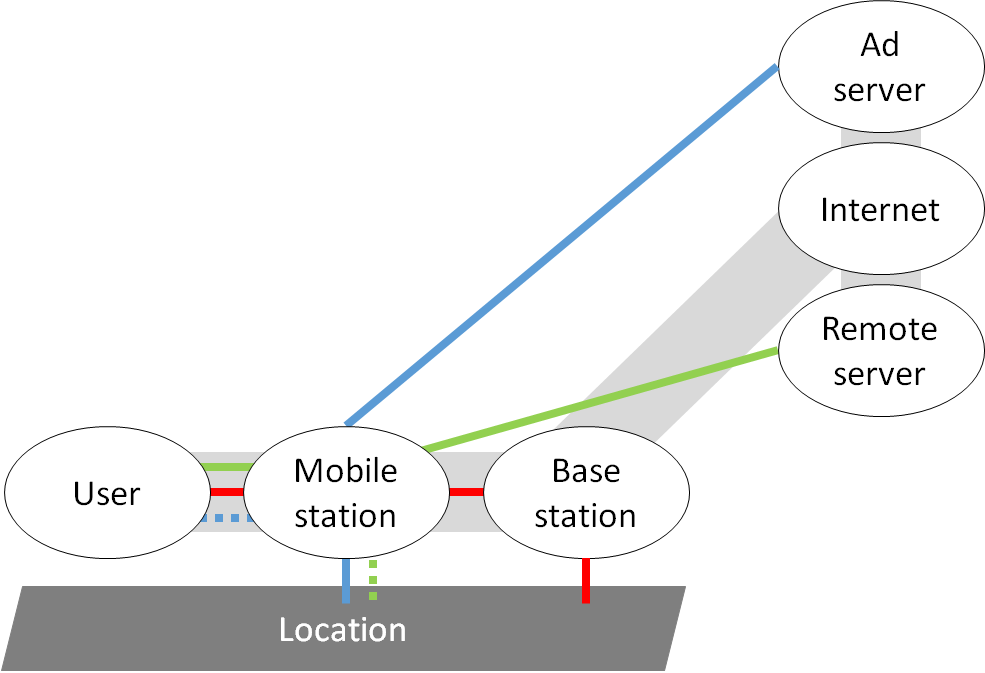
\includegraphics[width=\textwidth]{graphics/attacks}
	\caption{Exposure of information that may result in potential vulnerabilities in location privacy. The user, mobile device, and base station are in some physical location. The thick gray line indicates the communication path between a user and a service. Solid colored lines indicate links known to a potential attacker. Dotted colored lines indicate links that may be inferred by an attacker. Red lines indicate information known to a service provider; blue an advertising client; and green a web service.}
	\label{fig:overview}
\end{center}\end{figure}

There are many ways people remain connected to the Internet, such as Wi-Fi, cellular network, and cable. In each of these cases, the time and location of a user connection is known to the service provider. There have been cases of IMSI-catchers being used dubiously to monitor individuals~\cite{dabrowski2014imsi}. Additionally, passive eavesdropping techniques may intercept any mode of wireless signal, including Bluetooth, allow for a varying degree of granularity to localize an individual. We need a flexible framework to model these types of attacks. Such a framework would allow us to measure and quantify wireless geolocation privacy with varied settings and attacker models. 

There are many attack vectors on a user's location privacy. Figure~\ref{fig:overview} diagrams the potential vulnerabilities from different classes of attackers. In Chapter~2, I look at a web service attacker. This service has information about who the user is and which device she is using, and may infer the location of the device (green lines). In Chapter~3, I look at advertiser attackers, who have information about the device's location, and may infer who the user is (blue lines). In Chapters 4 I look at service provider attackers, and how to defend against them. These attackers have concrete information about the user, device, and location, so we must break the link between user and device (red lines). 

The following is a general framework that uses trajectory linking to improve location profiling. For simplicity, the following equations do not take into account the time of day, and other factors that may help determine the user of a trace. It contains no details about the location profiling and trajectory linking themselves.

\paragraph*{Model}
Let $U$ be the users in our database. These are users for which we have some location history data $S_U$.
Let $S^*$ be all sequences of locations $L$ within some time range of interest.
A sequence $\mathbf{s}\in S^*=s_0,\dots; s_i\in L$.

The most likely user given an anonymous sequence of locations is
\begin{equation}
\arg\max_up(u|\mathbf{s}),
\end{equation}
where 
\begin{equation}
p(u|\mathbf{s}) = p(u|s_0,\dots).
\end{equation}

We can determine the most likely path for a user as
\begin{equation}
\arg\max_\mathbf{s} p(\mathbf{s}|u).
\end{equation}

Trajectory linking is the most likely sequence given another sequence:
\begin{equation}
\arg\max_\mathbf{s} p(\mathbf{s}|\mathbf{s'}).
\end{equation}

Finally, we can determine the most likely user of a sequence using information from possible additional trajectories. 
Let $Z^s$ be the permutation of paths in $S^*$ that are linkable to $s$ (i.e., there is no overlap in time, and no impossibly fast transitions), then
\begin{equation}
p(u|\mathbf s) = \sum_{z\in Z^{\mathbf s}} p(z|\mathbf s) p(u|z).
\end{equation}
Generating a permutation of paths and computing their probability is intractable for many tests, so we may use heuristics to include only obvious links.

If an attacker wishes to deanonymize an entire anonymized database, they would want to determine the most likely matching of users to traces. 

We can determine the most likely corresponding (ordered) set of users $\hat{U}$, given some set of anonymous traces $S^{*'}\subseteq S^*$ as
\begin{equation}
\arg\max_{\hat{U}} p(\hat{U}|S^{*'}),
\end{equation}
where
\begin{equation}
p(\hat{U}|S^{*'}) = \prod_i p(\hat{U}_i|S^{*'}_i).
\end{equation}

To determine a set of users, given some anonymous set of traces, and consider possible links, we calculate
\begin{equation}
p(\hat{U}|S^{*'}) = \prod_i \big( \sum_{z\in Z^{S^{*'}_i}} p(z|S^{*'}_i) p(\hat{U}_i|z) \big).
\end{equation}

Accordingly, the $k$-anonymity of a user $u$, given a trace $s$, is 
\begin{equation}
k\textrm{-anonymity} = \textrm{rank}(\langle p(u|\mathbf{s}), u \rangle, U).
\end{equation}

\paragraph*{Linking algorithms}

There are effective, naive location profiling algorithms~\cite{de2008identification}. A simple location profiling algorithm can effectively determine the users of anonymous sequences. In the Reality Mining dataset~\cite{eagle2006reality}, 95 anonymous users could be deanonymized with 80\% accuracy (as I show in Chapter 4). % TODO: existing experiments with motifs
However, most trajectory linking algorithms have been intended for improving positioning or object tracking, rather than from an adversarial perspective~\cite{jaqaman2008robust,yang2012online,qin2012improving}. I investigate some trajectory linking strategies in this section.

I evaluated two methods of linking using traces of 300\,000 cell phone users in a particular country\footnote{I was unable to obtain permission to publish using this dataset; thus, I have abandoned these results, and will have to find an alternative for my thesis.}, tracked two weeks at a time. Each user had a log of which location area code (LAC) among 1\,666 they were present in every ten minutes.

\emph{Motifs.} Because the dataset had only 1666 LACs, the mobility data was very coarse. This means that our traces do not capture much mobility unless a user makes distant trips. I was unable to regular sequences of paths that are more than three locations. Among 100000 users, I was able to identify paths with 3-location trajectories linked once with another (6 locations long) with 40\% accuracy. Note that the existence of these trajectories were exceptionally sparse in this dataset.

\emph{Estimated link frequency.} To estimate the likelihood of a link occurring, we count the frequency of a link (i.e. a transition from location $a$ to $b$) in the dataset. 
Assuming
\begin{align}
	Count(AppearsTogether(a,b))&=Count(a) + Count(b),\label{eq:link}\\
	\textrm{then } E[p(a\rightarrow b|a,b)] &= \frac{Count(a\to b)}{Count(a)+Count(b)}\label{eq:link2}
\end{align} 

However, it may be the case that $a$ and $b$ rarely appear together (in time). For example, $a$ may appear a lot more than $b$, but $b$ often transitions from $a$. This breaks the assumption in Equation~\ref{eq:link}. We can make the assumption that the probability $b$ comes from $a$ and $a$ goes to $b$ is similar when they appear together as when they do not, in which case, we have 
\begin{align}
\label{eq:link3}
	E[p(a\rightarrow b|a,b)] &= \frac{p(a|b)*p(b|a)}{p(b)*p(a)}
\end{align}
% TODO: fix this, maybe

The results from this linking method is shown in Figure~\ref{fig:linkcdf}.
\begin{figure}\begin{center}
		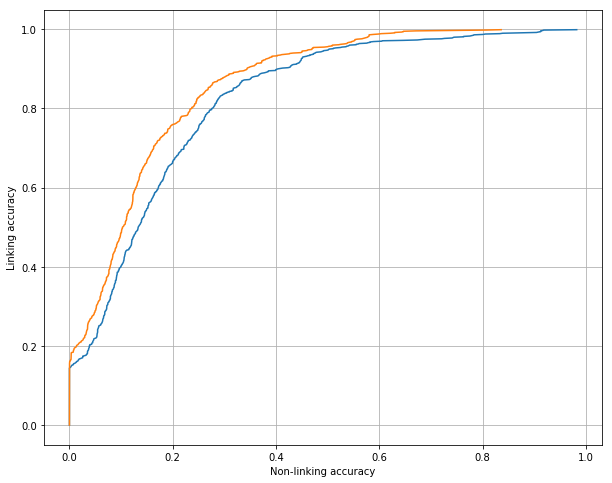
\includegraphics[width=0.7\textwidth]{graphics/linking2}
		\caption{The $x$-axis represents accuracy of identifying a set of traces unlinked, and the $y$-axis represents the accuracy of the same set linked based on Equation~\ref{eq:link3}. Red is a link before, and blue is a link after.
		\label{fig:linkcdf}}
\end{center}\end{figure}

% TODO: better caption or label
\begin{figure}\begin{center}
		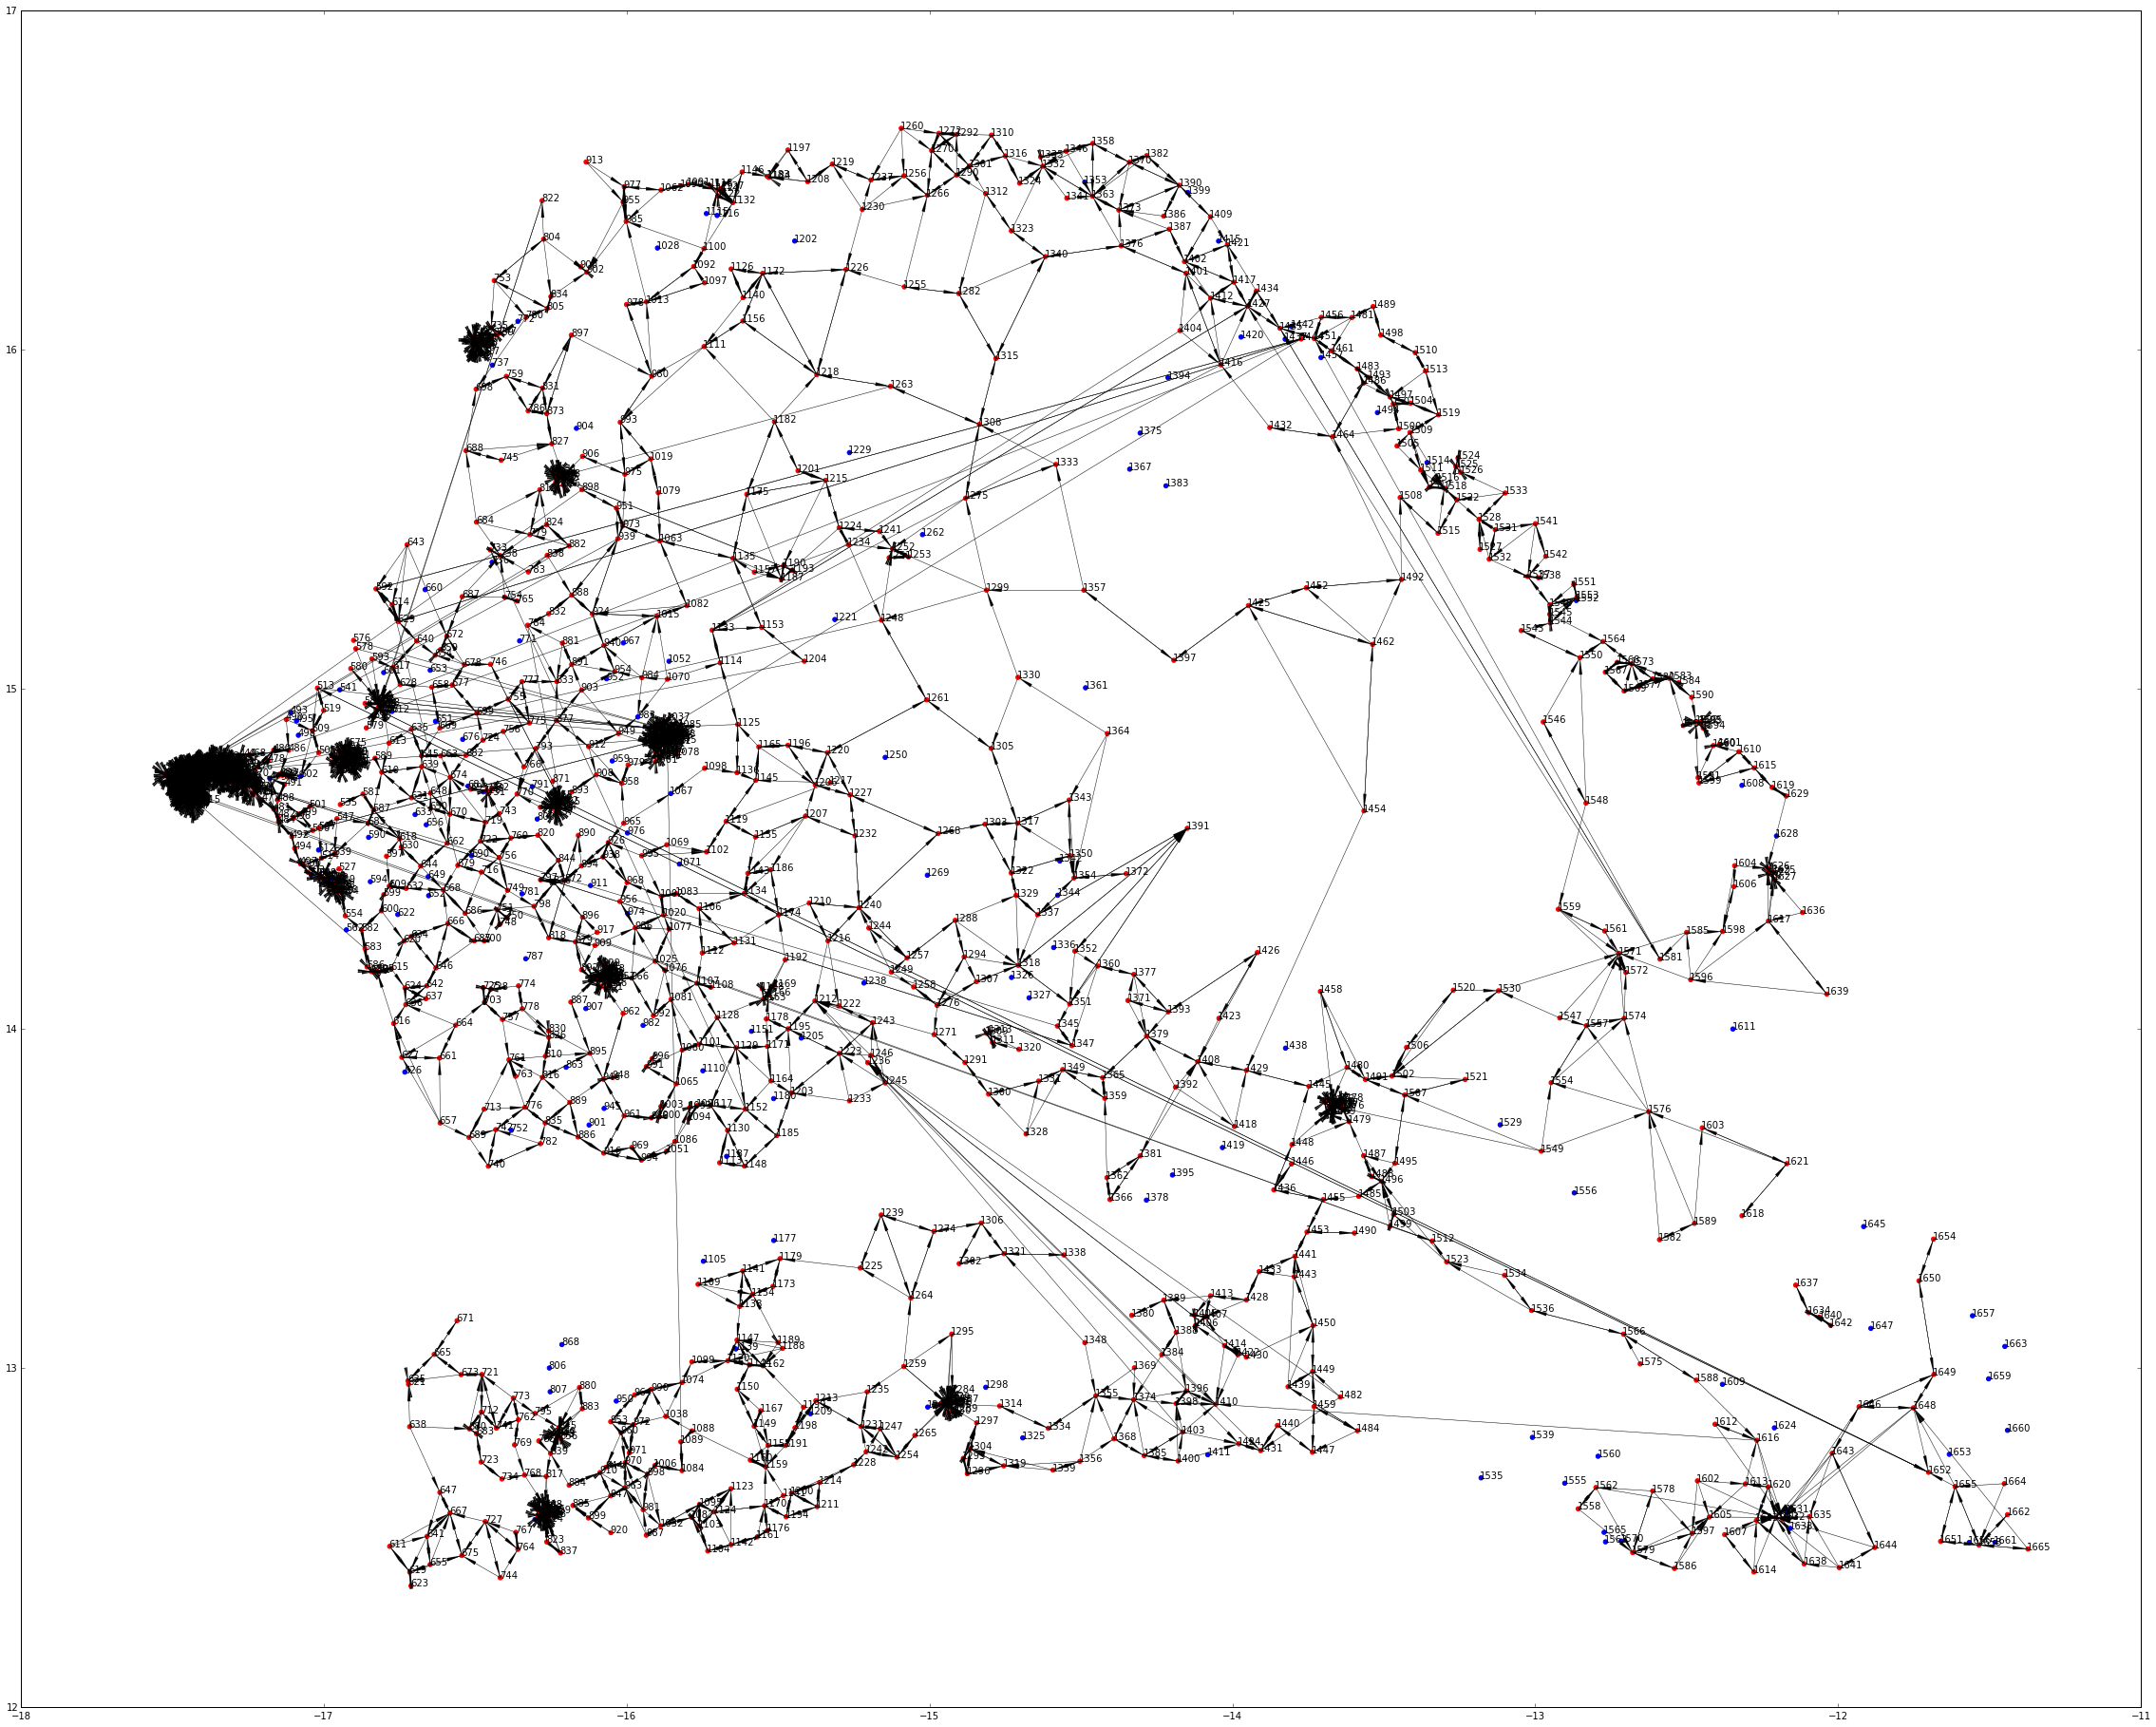
\includegraphics[width=\textwidth]{graphics/senegalmap}
		\caption{Most common LAC transitions in Senegal. Longer lines may indicate trips by air or sea.
			\label{fig:senegal}}
\end{center}\end{figure}

Multiple target tracking (MTT) algorithms\cite{nillius2006multi} can be used as heuristics for trajectory linking. Because the dataset above contains only coarse data on time and physical location, MTT would be ineffective. To simulate the finer-grained location data that a cell tower would have, I use a dataset tracking over 300 taxis in the Rome metropolitan area over a month\cite{cunha2015understanding} to evaluate the effectiveness of a naive MTT algorithm\footnote{\url{http://soft-matter.github.io/trackpy}} for trajectory linking, assuming no points are linked initially. Figure \ref{fig:mtt} shows that if location is updated constantly, taxis would still be identified with 40\% accuracy without any initial linking.

% TODO: self mixing, breaking links

% TODO: fix legend --- area of thing
\begin{figure}\begin{center}
	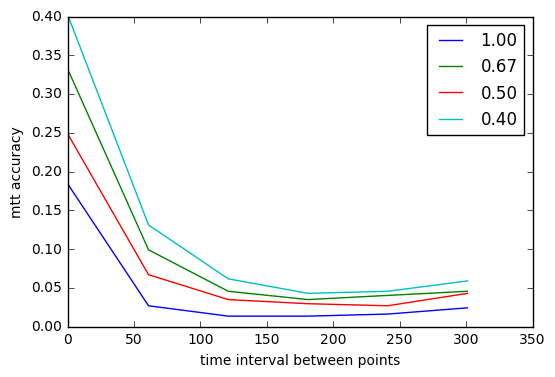
\includegraphics[width=0.7\textwidth]{graphics/mtt}
	\caption{MTT accuracies for 374 taxi drivers around Rome over a period of 20 minutes. Colors represent different relative granularities.}
	\label{fig:mtt}
\end{center}\end{figure}

%% TODO: stuff for Mariya
%% TODO: linking algo for the D4D data


\section{Proposed work: Fully implement a utility model and collect data to rigorously evaluate it}
%\paragraph*{Utility-privacy framework}

I was able to pilot trajectory linking and location profiling using several datasets; however, these datasets are insufficient to evaluate any algorithm (and one has not given us permission to publish). Additionally, many datasets are either old, crowd-sourced, or have been fuzzed with noise. To extend this chapter, I propose to answer a few key questions:
\begin{enumerate}
	\item What are some properties of the wireless topology on a cell phone network in a rural or urban area? Knowing these properties would allow me to more accurately synthesize and validate a dataset.
	\item How effective are LP/TL algorithms in de-anonymizing traces?
	\item What is the utility cost to avoid being tracked by these algorithms?
	% \item What is the efficacy and complexity of LP/TL methods?
	% \item How effective are these methods after excluding low-value locations such as home and work?
	% \item How useful is information about wireless topology in LP/TL algorithms?
\end{enumerate}

To answer these questions, I will first do field surveys of the Amherst and Boston areas, to determine the density of cell towers and physical locations served. If I am able to recruit enough users, I will track how often a phone connects to the network to make a call. The call data in particular will be useful in Chapter~4. 

Using this information, I will synthesize a larger dataset of mobility traces and calls, and validate this against any additional datasets I find. I will use these datasets to develop and evaluate several location profiling or trajectory linking algorithms. 

Finally, I plan to develop a model to measure the balance between utility and privacy. I will alter traces in the aforementioned datasets to simulate evasive reduction of phone usage, and analyze the trade-off between usability and privacy. I will pay special attention to how much significant stays like home or work may make a use significantly more identifiable, but is information that is of little value to both targets and attackers. An economic model may better encapsulate these possibilities, if a user can assign different values to different locations.

% Previous work has used $k$-anonymity, or $(k, p)$-anonymity as a privacy metric\cite{shou2013supporting}. Instead, we use the economic measure of utility as a metric for two reasons: (1) it allows us to balance the cost of utility with the cost of privacy loss, and (2) it allows us to assign different values to different locations. For example, a user could have "significant stays" at home and work, a place where they would likely be identified, anyway, so achieving location privacy here is not worth it if they are able to change identities without being easily linked once they leave work.

% I plan to adapt the framework above for use in an economic model of privacy, as well as compare it against other known models for privacy\cite{shokri2011quantifying,shin2012privacy}. I plan to implement more sophisticated location profiling and trajectory linking algorithms to work with the framework. I will also do a field survey by sending phones around the Amherst area and collecting information about cell phone towers, signal strength topology, and synthesizing a dataset to evaluate these algorithms. 